\documentclass[11pt]{amsart}
\usepackage{geometry}                % See geometry.pdf to learn the layout options. There are lots.
\geometry{letterpaper}                   % ... or a4paper or a5paper or ... 
%\geometry{landscape}                % Activate for for rotated page geometry
\usepackage[parfill]{parskip}    % Activate to begin paragraphs with an empty line rather than an indent
\usepackage{graphicx}
\usepackage{amssymb}
\usepackage{epstopdf}
\usepackage[colorlinks=true, pdfstartview=FitV, linkcolor=blue, 
            citecolor=blue, urlcolor=blue]{hyperref}
\DeclareGraphicsRule{.tif}{png}{.png}{`convert #1 `dirname #1`/`basename #1 .tif`.png}

\graphicspath{{figs/}}

\begin{document}

\begin{center}
\huge{\textbf{Vaximap: optimal delivery of housebound vaccinations}}

\large{Thomas Kirk\textsuperscript{1}, Adam Barker\textsuperscript{2}, Armen Bodossian\textsuperscript{3}, Robert Staruch\textsuperscript{1}}

\small{1 Institute of Biomedical Engineering, Department of Engineering Science, University of Oxford\\
2 Something\\
3 Something}

\end{center}

\section{Abstract}

\section{Introduction}

There are estimated to be around one million housebound patients in the UK. During the Covid-19 vaccination campaign, responsibility for inoculating these patients has rested with individual GP surgeries. Given that these patients are more likely to be in one of the nine priority groups identified by the JCVI, reaching them in a timely and efficient manner is a key component of the success of the overall campaign. 

From a delivery perspective, the core logistical challenge of vaccinating housebound patients is determining the fastest order in which to visit the individuals. This is an example of the travelling salesman problem, which has been extensively studied in the domain of computer science. Notwithstanding the existence of algorithms to solve the travelling salesman problem \cite{X}, vaccination imposes some extra constraints. Firstly, because there are a fixed number of doses in a vial, it is preferable to sort patients into groups sized of this same number. This ensures that exactly one vial of vaccine will be required for each group of patients visited, which minimises wastage. Secondly, due to the storage requirements of the vaccines themselves (in particular storage temperatures), visiting patients in the fastest order minimises the time that vials spend outside of the cold chain, which further minimises wastage. 

In response to a call for help from GPs and practice managers on Twitter, Vaximap was set up in January 2021 to automate the process of planning housebound vaccinations. Users need only upload an Excel spreadsheet containing anonymous patient identifiers and postcodes (which may easily be exported from an EMIS database) and specify some constraints. The service then sorts the patients into a number of groups, finds the optimal visiting order within each group, and provides easy-to-follow directions in both email and spreadsheet form. The service is provided free of charge for all users at \url{https://vaximap.org}. 

\section{Implementation}

\begin{figure}[htbp]
\centering
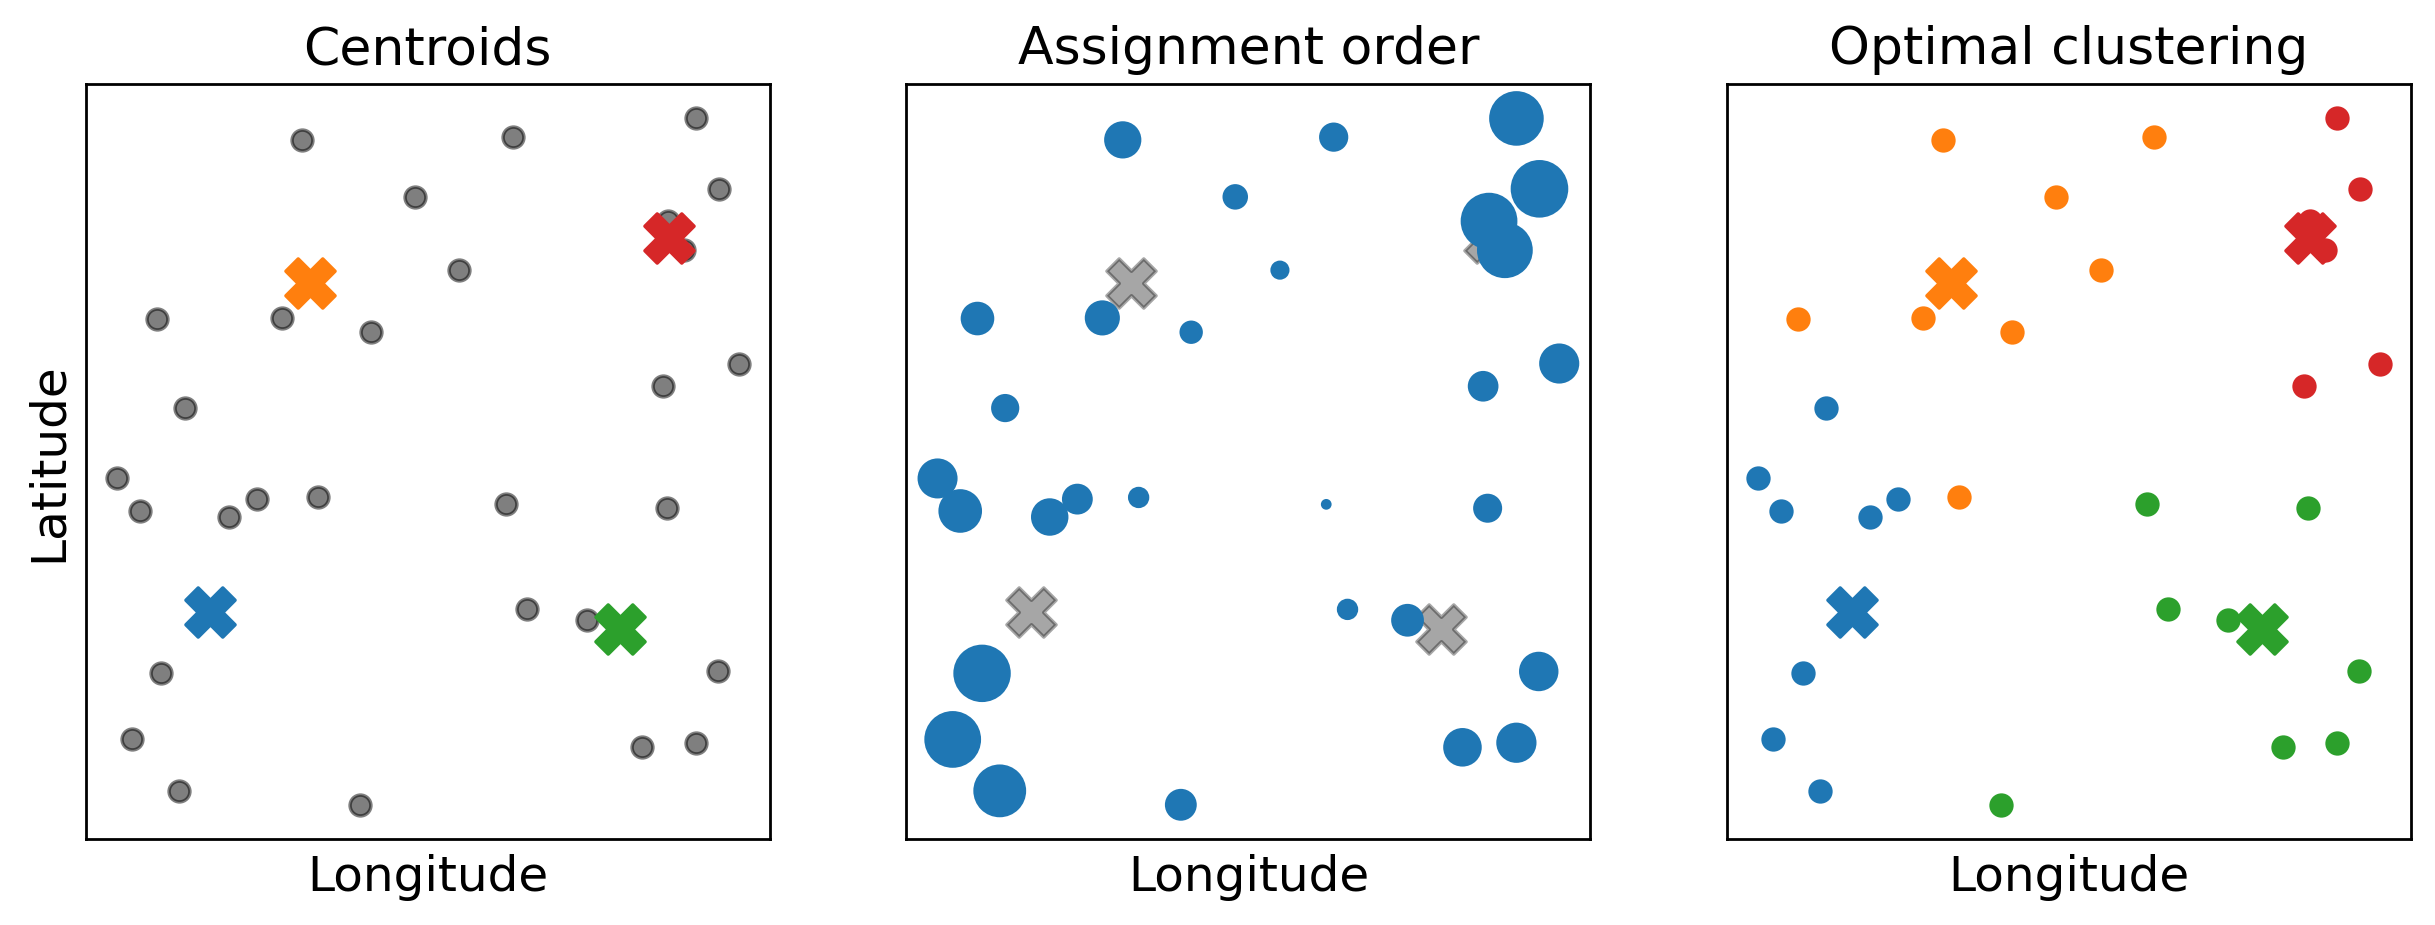
\includegraphics[width=\textwidth]{clustering_demo.png}
\caption{Example clustering of 30 patients into groups of eight. Left: initialisation of four cluster centroids (denoted with X). Centre: order of patient assignment, where larger circles indicate a greater optimisation penalty. Patients in the centre of the plot could be assigned to any cluster with low cost, so are dealt with last. Right: the optimal clustering of patients after assignment. The red cluster has six patients due to imperfect number division.}
\label{default}
\end{figure}


The problem is posed as sorting $N$ patients into a number of groups, of fixed size $D$, and determining the fastest order in which to visit the patients of each group. The postcode for each patient is converted into a latitude and longitude coordinate via the use of Microsoft Bing’s geocoding services \cite{X}, such that there are $N$ coordinates on the $x,y$ plane that need to be visited. 

For simplicity, it is assumed that the constraint on group size $D$ is set by the user to be the number of vaccine doses in a vial (for example, nine for Oxford-AstraZeneca), though in practice any number between 3 and 25 can be used. It follows that the $N$ patients must be sorted into $G = \mathrm{ceil}(N / D)$ groups (this quantity must be rounded up in the case that $D$ does not divide perfectly into $N$, in which case one group will have size less than $D$). 

The next step is to group the patients such that they are proximal in space, which will ensure that the travel time within each group is minimised. The $k$-means clustering algorithm \cite{X} provides a general means of grouping an arbitrary number of points into a fixed number of groups based on proximity, however it suffers the drawback of not enforcing any constraint on group size. For example, though it can sort $N$ patients into $G$ groups, there is no guarantee that each of these groups would be sized $D$ or smaller. As such, a modified form referred to as \textit{iterative k-means} clustering is used instead \cite{X}. 

Under this modification, an initial grouping of the $N$ patients into $G$ groups is performed using standard $k$-means. The group centroids (centre coordinates of each group) are extracted but the groupings themselves discarded. The $N$ patients are sorted in order of descending optimisation penalty, defined by the quantity (distance to furthest group centroid – distance to nearest group centroid). Qualitatively, this sorting will place those patients that are near to only one centroid first, whereas patients that are approximately equidistant from multiple centroids will be placed last. Finally, the patients are sequentially allocated in this order: each patient will be allocated to the centroid to which it is closest, that is not already full (ie, size equal to $D$). 

After these steps, the initial set of $N$ patients have been sorted into $G$ spatially proximate groups. Route directions for visiting the individual patients in the optimal within-group order are obtained via Microsoft Bing’s mapping API, making use of the optimise waypoints facility \cite{X} (the API imposes a limit of 25 patients on group size). This step, which is performed entirely in the cloud, makes use of existing solutions to the traveling salesman problem. Optionally, the user can specify a fixed start and end point for their routes (for example, the address of their GP surgery); each route will then be a round-trip from that location. Similarly, routes can be provided for either driving or walking (the latter useful in the urban environment). 

\section{Analysis}

As of June 2021, Vaximap has been used to plan delivery for over 301k patients. 

\section{Discussion}

\section{Conclusion}

\end{document}  